\chapter{Use case: Lattic ECP5}
We will apply our algorithm to map virtual FPGAs to the concrete Lattice ECP5 FPGA. An image of this FPGA on an evaluation board is shown in Figure \ref{fig:evaluationboard}. This FPGA's architecture consists of `tiles' of different types in a grid pattern. Each of these tiles has an associated x- and y-coordinate in the grid system and is (generally) topologically the same as tiles of the type elsewhere in the grid. There exists I/O tiles which' function is to retrieve and send data from outside the FPGA, DSP tiles that perform signal processing calculations, tiles that only provide routing structure, RAM tiles and tiles that are internally used for clock management and configuration.

The structure of an ECP5 FPGA is shown in Figure \ref{fig:ecp5architecture}. This figure shows the grid/tile structure of the ECP5 along with specific components from the electrical engineering domain. The largest portion of the grid structure are logic tiles that contain 8 LUTs and 8 registers (or flip-flops (FF)), bundled in 4 modules. We will focus on this type of tile to find homeomorphisms. We used Project Trellis\cite{todo} to obtain graphs of both an individual tile (shown in Figure \ref{fig:ECPTGephi}) and of collections of adjacent tiles.

The virtual FPGA we aim to emulate on this board (which we will call \textit{VirBoard}) is one that, like the ECP5 consists of a tile-like structure with no wires spanning no more than a single tile. Because of this limitation, a student may freely drag-and-drop functionality in the virtual environment without worrying about implicitly overlapping connections. Each tile in this virtual FPGA has significantly less functionality than one of the ECP5. It has a single in- and output at each compass direction, a 2-bit LUT and an 1-bit register. It can be configured in several ways:

\begin{enumerate}
\item As a single wire from one compass direction to the opposite
\item As a cross-section of two orthogonal wires
\item A wire from direction A making a 90 degree turn to direction B, and a wire from direction B to the opposite direction of A.
\item As a configurable 2-input-2-output LUT with any two compass directions as inputs and the other two as outputs
\item As an 1-bit register with any compass direction as data input, any other compass direction as clock-enable (allowing the register value to be set) and any single remaining compass direction as register output. The final compass direction outputs the input of the register.
\end{enumerate}

There are countless ways to model this functionality using wires, transistors and logic cells, each of which would yield working emulations if a subgraph homeomorphism of the model is found in the graph model of the concrete FPGA. In principle, one could enumerate all such models and attempt to find subgraph homeomorphisms with each of them, maximizing the expected result. For the scope of our research, however, we limit ourselves to a single graph model that performs well for subgraph homeomorphism search. For this purpose, we design the model of the virtual FPGA with two goals in mind:

\begin{enumerate}
\item It contains as few vertices and edges as possible, so that the search space is as small as possible.
\item It contains as few rare resources as possible, so that more subgraph homeomorphisms are present.
\end{enumerate}

We designed a graph model of VirBoard that encompasses all listed functionality and contains a total of 30 vertices and 32 edges. We were not able to produce a smaller model or one that uses fewer resources. This graph model of VirBoard is shown in Figure \ref{fig:virboard}.

\begin{figure}
\centering
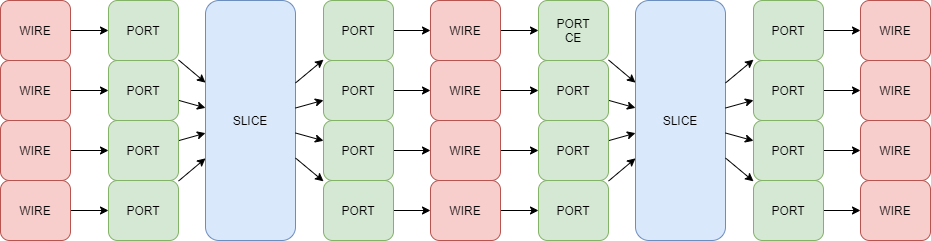
\includegraphics[width=0.8\textwidth]{images/virtualFPGA2.png}
\caption{A graph model of a single cell of the virtual FPGA aimed to emulate on the Lattice ECP5}
\label{fig:virboard}
\end{figure}	


\begin{figure}
\centering
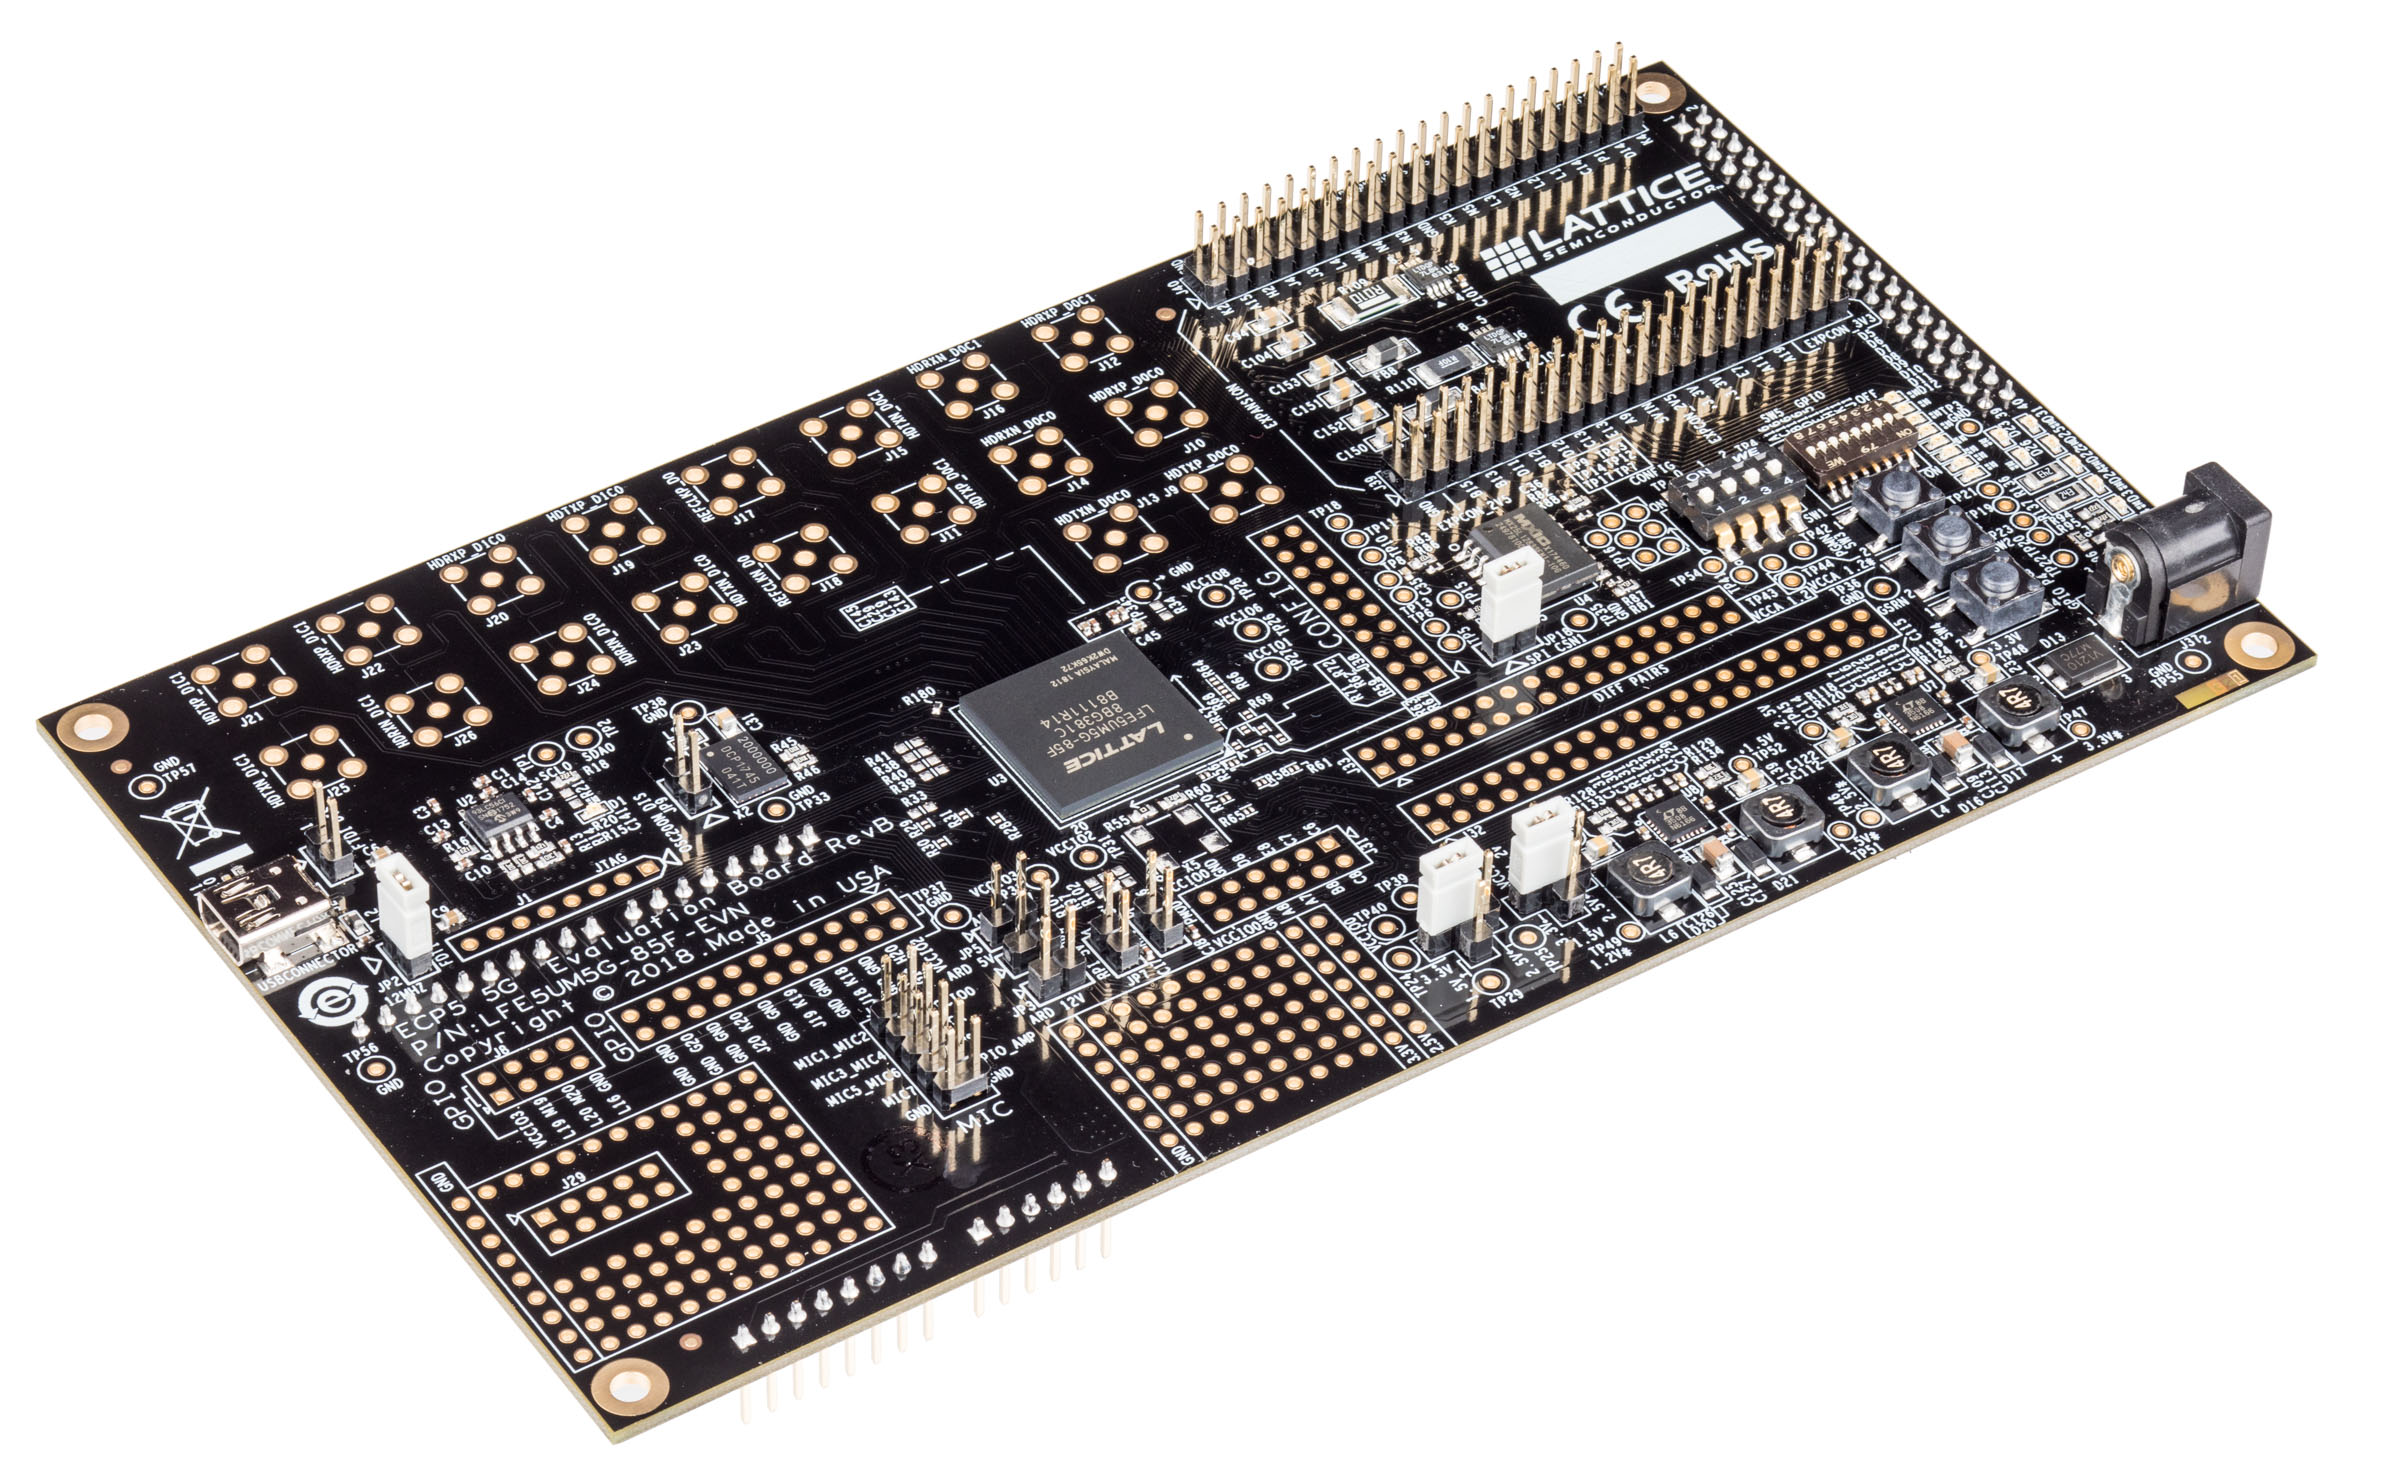
\includegraphics[width=0.5\textwidth]{images/ECP5.png}
\caption[Evaluation board of the LFE5UM5G-85F FPGA: a variant of the ECP5.]{Evaluation board of the LFE5UM5G-85F FPGA: a variant of the ECP5.\footnotemark}
\label{fig:evaluationboard}
\end{figure}
\footnotetext{\texttt{http://www.latticesemi.com/products/developmentboardsandkits/ecp5evaluationboard}, accessed July 10th 2020}	


\begin{figure}
\centering
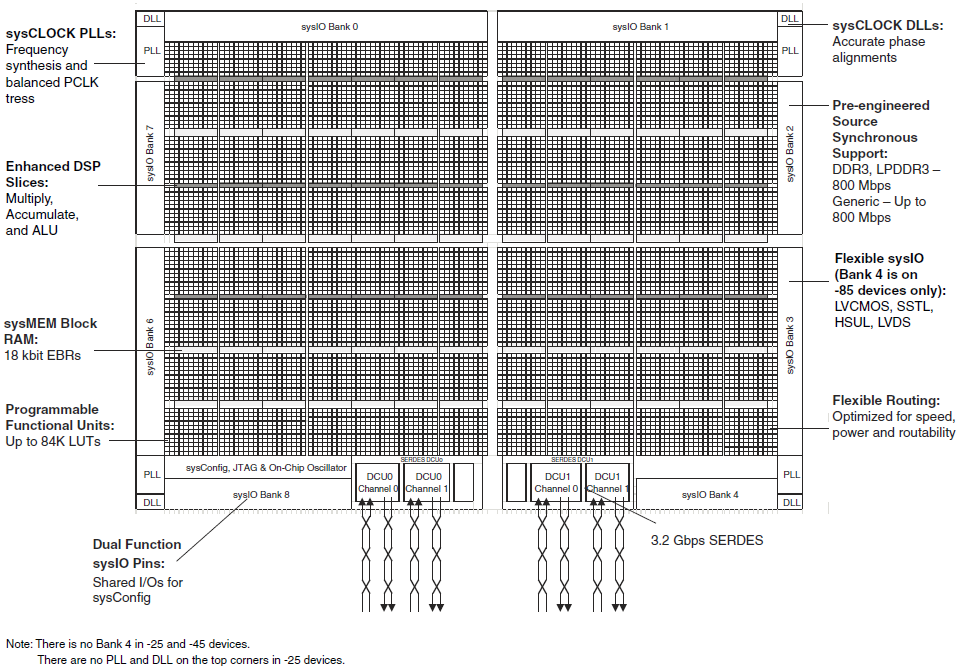
\includegraphics[width=0.8\textwidth]{images/ECP5Architecture.png}
\caption[Architecture of the ECP5 FPGA. Note that it is tile-based in a square grid structure, just like VirBoard.]{Architecture of the ECP5 FPGA. Note that it is tile-based in a square grid structure, just like VirBoard.\footnotemark}
\label{fig:ecp5architecture}
\end{figure}
\footnotetext{ECP5\texttrademark and ECP5-5G\texttrademark Family Data Sheet (FPGA-DS-02012 Version 1.9), accessed October 1st 2020}	

\begin{figure}
\centering
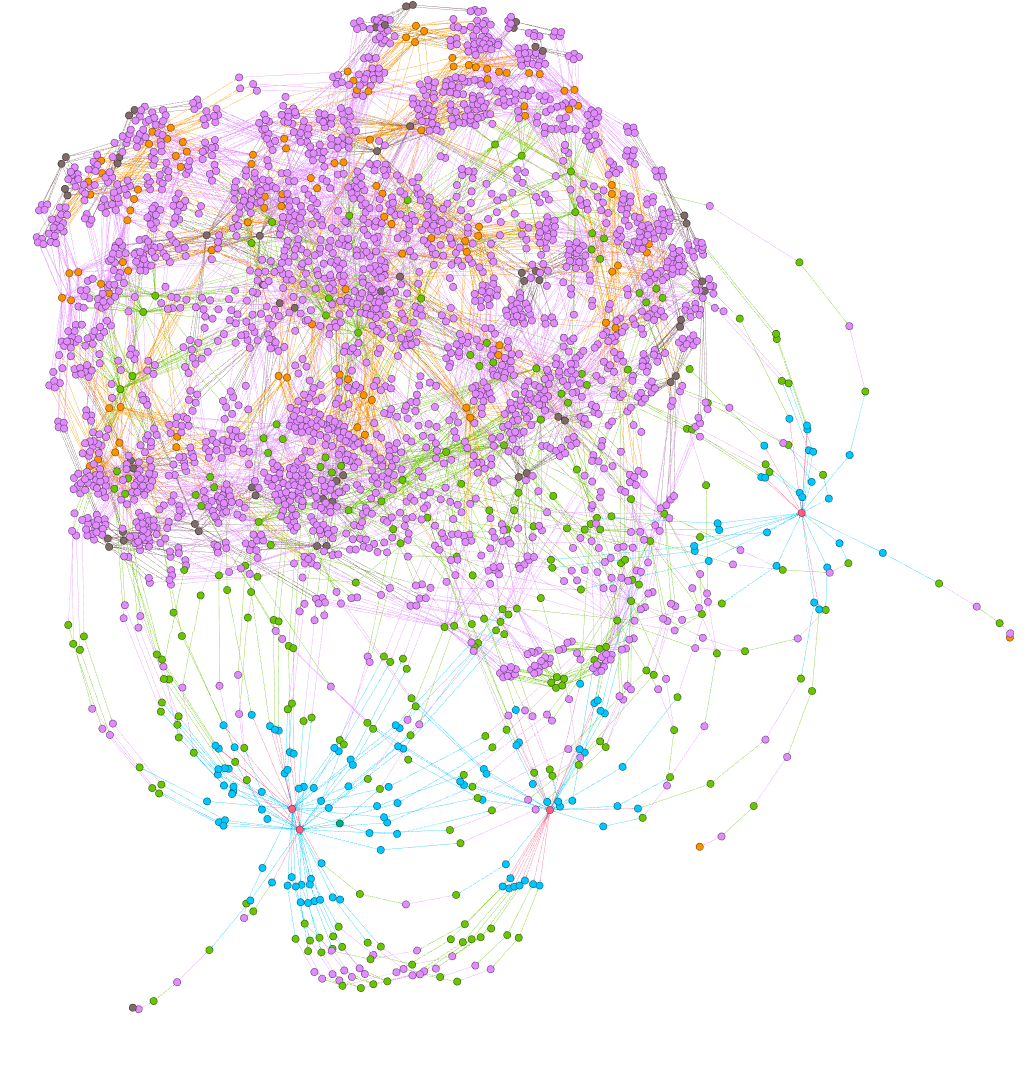
\includegraphics[width=1\textwidth]{images/gephiScreenshot.png}
\caption{Graph model of a single ECP5 logic tile (out of $\pm$42000 logic tiles). Transistors are purple, logical units are red, ports are blue, wires are orange (except those that are neighbouring an adjacent cell, which are brown).}
\label{fig:ECPTGephi}
\end{figure}



